\chapter{Estado del Arte\label{sec:EstadoDelArte}}

Con el paso del tiempo se ha demostrado que una de nuestras mayores virtudes como seres humanos es la habilidad de aprovechar el saber cultivado por otras personas para realizar nuevos descubrimientos con mayor facilidad. En la actualidad con la ayuda de Internet esta ventaja se ha visto potenciada hasta límites insospechados.

Como se ha mencionado con anterioridad en el capítulo \ref{sec:introduccion}, a lo largo de los años se han desarrollado numerosas alternativas a los dispositivos presentes en los hospitales y laboratorios utilizados normalmente para el estudio del cerebro. 
\\Aunque se han invertido muchos recursos en estos dispositivos, el objetivo es permitir ampliar el número de personas capaces de estudiar el cerebro humano, consiguiendo  así aumentar las posibilidades de mejorar nuestro conocimiento sobre el mismo.

De esta forma debería ser más fácil realizar nuevos descubrimientos como, por ejemplo, encontrar nuevas formas de diagnosticar enfermedades o de realizar una comunicación hombre-máquina para aquellas personas que por un motivo u otro no pueden utilizar los medios convencionales.

\clearpage

\section{Dispositivos similares\label{sec:Disp_similares}}

A lo largo de este capítulo se presentarán algunos de los dispositivos capaces de capturar un EEG haciendo uso de electrodos, algunos a nivel personal, otros enfocados a la docencia y, por supuesto, algunos diseñados por empresas con el fin de realizar un producto final que vender a terceros.

\subsection{Proyectos personales\label{sec:Pro_personales}}

En internet se pueden encontrar algunos ejemplos de personas que han dedicado su tiempo a crear dispositivos capaces de captar un EEG. 

\subsubsection{Instructables}

La página web \textbf{instructables.com} ha propuesto a sus usuarios la creación de un sistema de adquisición de EEG y ECG sencillo y barato. El dispositivo final resulta muy interesante, pues con unas pocas resistencias, condensadores y un par de amplificadores operacionales son capaces de montar un dispositivo funcional. La figura \ref{} muestra el esquemático final del dispositivo.

\begin{figure} [h]
    \centering
    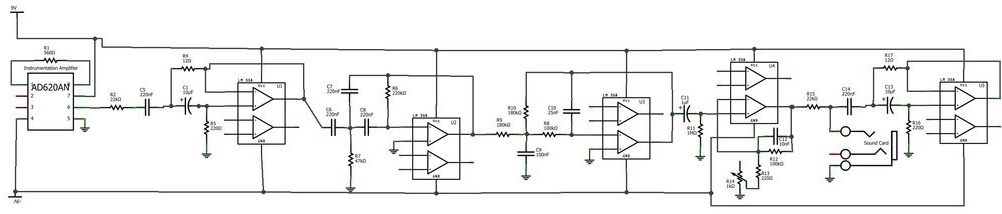
\includegraphics[width=13cm]{EdA_EEG_0}
    \hfill
    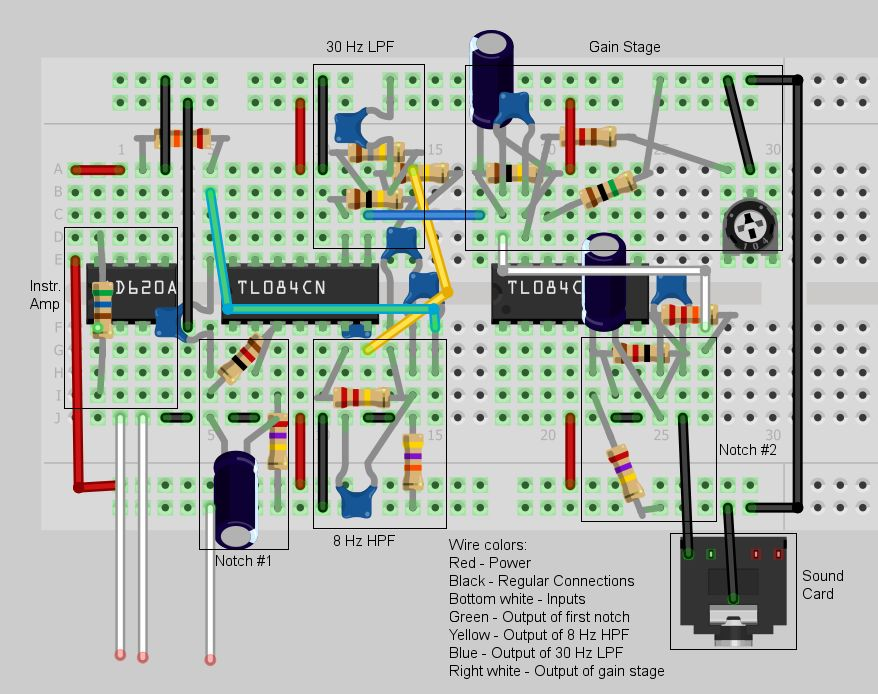
\includegraphics[width=9cm]{EdA_EEG_1}
    \caption{Esquema electrónico casero para la captura de un EEG \cite{DIY_EEG}}
    \label{fig:EdA_EEG_1}
\end{figure}

Este sistema es muy interesante y para fines educativos cumple perfectamente su función pero tiene en cuenta el ruido que afecta a la señal ni otras características importantes como son el aislamiento del paciente de la red eléctrica.

\subsubsection{OpenEEG}


\begin{figure}[h]
  \begin{subfigure}[b]{7cm}
   	\centering
    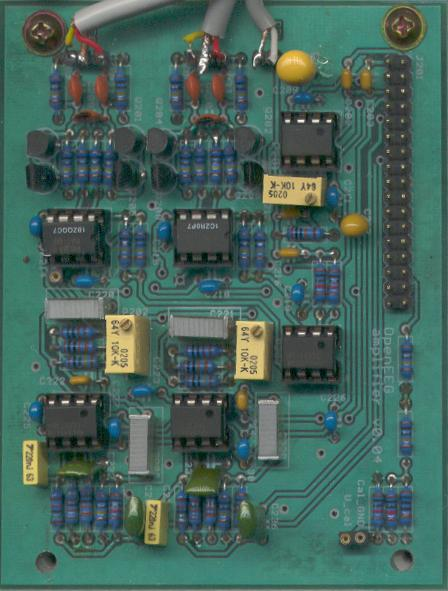
\includegraphics[width=7cm]{Openeeg_amp_l}
    \caption{Tarjeta de adquisición}
    \label{fig:Openeeg_amp_l}
  \end{subfigure}
  \hfill
  \begin{subfigure}[b]{7cm}
  	\centering
    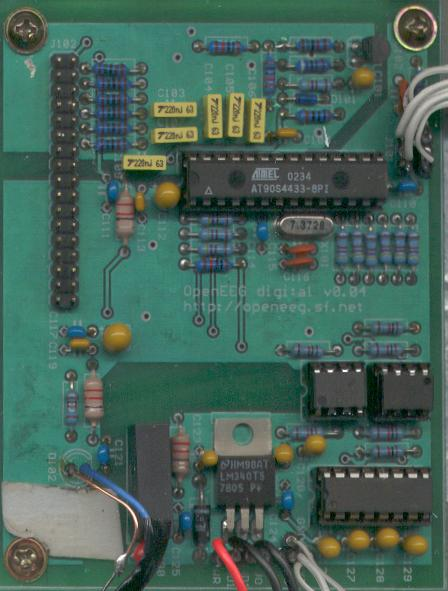
\includegraphics[width=7cm]{openeeg_digital_l}
    \caption{Tarjeta de procesado}
    \label{fig:openeeg_digital_l}
  \end{subfigure}
  \caption{Elementos que conforman OpenEEG}
  \label{fig:OpenEEG}
\end{figure}


\subsubsection{Beanie}

Esta curiosa iniciativa utiliza un analizador de EEG acoplado a un gorro para que este se ilumine en función del estado y concentración de la persona.

\begin{figure} [h]
    \centering
    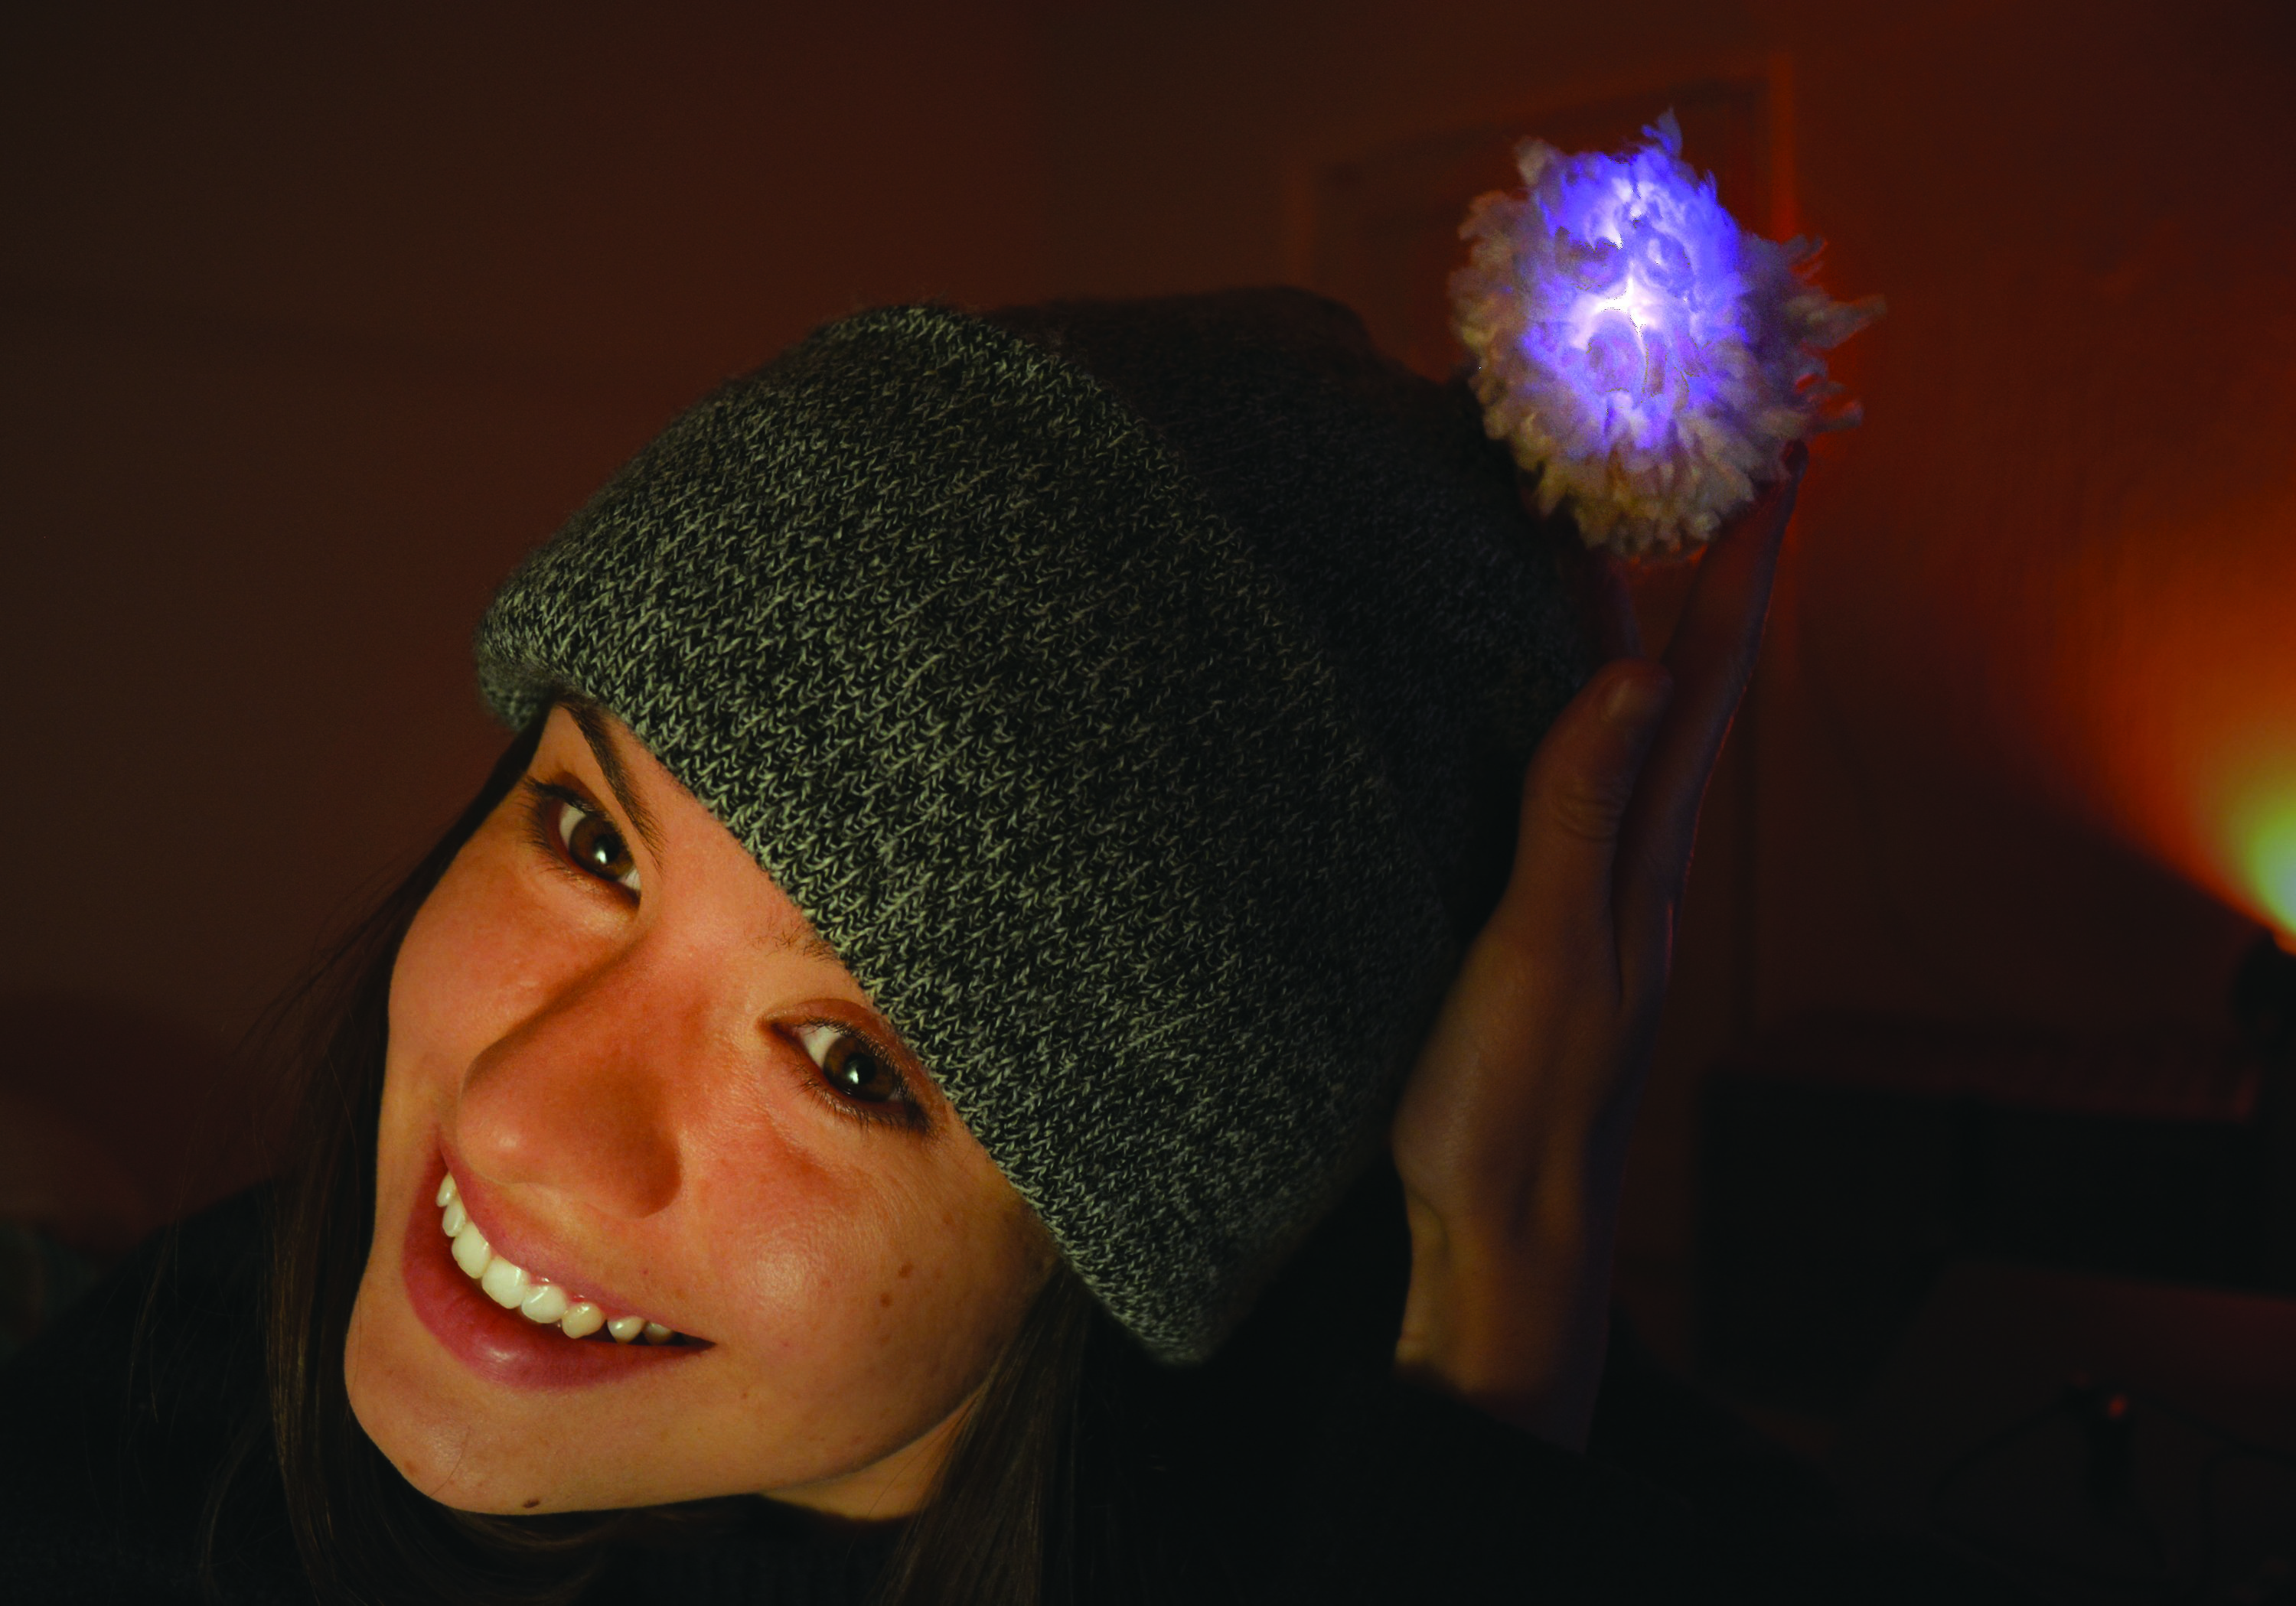
\includegraphics[width=7cm]{EdA_Beanie}
    \caption{Beanie en funcionamiento}
    \label{fig:EdA_Beanie}
\end{figure}

El funcionamiento es muy similar al resto de dispositivos ya explicados: se adquieren señales desde electrodos situados en la cabeza, se filtra la señal para eliminar el ruido y se presenta al usuario.

Para la adquisición de la señal utiliza un chip de la compañía Neurosky llamado ThinkGear ASIC Module que tiene integrado un sistema de adquisición y filtrado de señales. Posteriormente está se transfiere a un módulo TinyLily de Arduino que se encargará de realizar un segundo procesado para iluminar el pompón del gorro de la forma deseada.

El dispositivo se monta con relativa facilidad (1-2 días) y su precio ronda los 130€.

Hablar de los códigos accesibles en distintas páginas web, github y otros sitios.

Explicar que me he basado en ellos para agilizar el diseño ya que las definiciones de los distintos registros son similares.

\subsection{Proyectos docentes\label{sec:Pro_docentes}}

Hablar del de Nerea, como se ha trabajado con el y en que se basa.

\subsection{Comerciales\label{sec:Pro_empresa}}

Ejemplos comerciales como zanna u otras empresas.

Sistemas BCI comerciales.

Claramente todos los ejemplos anteriores presentan un coste bastante dispar entre ellos costando desde los cientos de euros de los proyectos personales y docentes hasta algunos miles de euros en el caso de productos comerciales.

Historia procesadores (Gráfica de procesadores)
Antecedentes de la placa (Open BCI)